\section{Continuity}\label{sec:continuity}

We identify a curvature profile with a vector $\kappa\in\R^n$ and a labelled
polygon with a vector $(P_i)_{i\in\Zn}\in\C^n$, with the product topologies.

\subsection{Local continuity}

\begin{theorem}\label{thm:local}
Let $n\ge4$ and let $\kappa^0\in\R^n$ be positive with a strict four-vertex
window~\eqref{eq:dfv}. There are an open neighbourhood $V$ of $\kappa^0$ and
$C^1$ maps $h\colon V\to\R^n$ and $P\colon V\to\C^n$ such that for every
$\kappa\in V$ the half-lengths $h(\kappa)$ realize $\kappa$ and $P(\kappa)$ is
the polygon developed from them by~\eqref{eq:vertices}, normalized by
$P_0=0$. In particular $P(\kappa)$ is simple, strictly convex and coherent,
with curvature $\kappa_i$ at every vertex.
\end{theorem}
% Lean: Gluck.Discrete.localContinuousRealization_of_dfv
%       (Gluck/Discrete/LocalContinuity.lean).

\begin{proof}
By Propositions~\ref{prop:reduction} and~\ref{prop:split} and
Section~\ref{sec:constructions}, $\kappa^0$ has a regular anchor, and
Theorem~\ref{thm:anchor-realizes} gives $V$ and $h$. The vertices
\eqref{eq:vertices} are real-analytic in $(\kappa,h)$, so $P$ is $C^1$. The
remaining properties are Section~\ref{sec:setup}.
\end{proof}

\subsection{No global continuous choice}

For $0\le s\le1$ consider the hexagon profile
\begin{equation}\label{eq:band}
  \kappa^{s} = (14,\ 11,\ 10+3s,\ 5,\ 7-3s,\ 3).
\end{equation}
Every $\kappa^s$ is positive and nonconstant. A direct check of all
quadruples of indices shows that the levels $c$ of strict four-vertex windows
of $\kappa^s$ form the set
\[
  (5,\,7-3s)\ \cup\ (11,\,10+3s),
\]
with an empty interval when the endpoints are reversed. The lower band is
nonempty for $s<2/3$ (window indices $0,3,4,5$), the upper band for $s>1/3$
(indices $0,1,2,5$). Hence every $\kappa^s$ is admissible and, by
Theorem~\ref{thm:main}, realized by a coherent convex hexagon.
% Lean: bandProfile_dfv_iff, bandProfile_admissible,
%       bandProfile_pointwise_realizable (Gluck/Discrete/GlobalContinuity)

\begin{figure}[t]
\centering
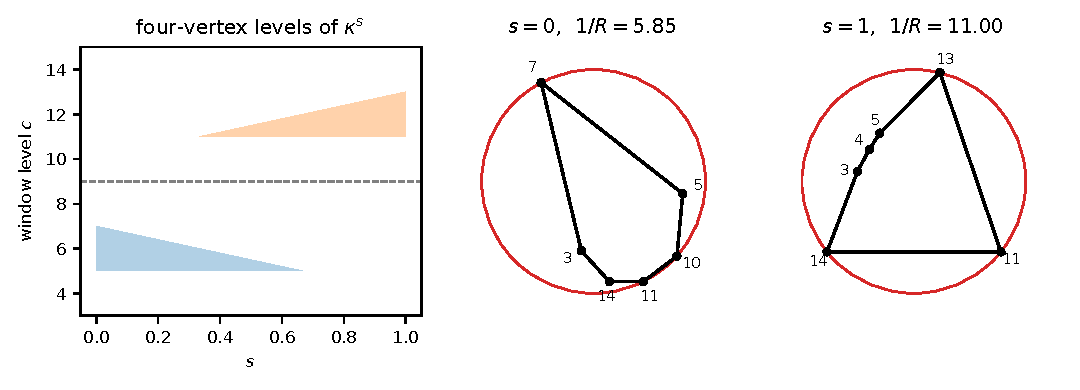
\includegraphics[width=0.8\textwidth]{tabachnikov/figures/hexagon.pdf}
\caption{Left: the levels of strict four-vertex windows of $\kappa^s$. Right:
realizing hexagons at $s=0$ and $s=1$ with their smallest enclosing circles.
The reciprocal enclosing radius is at most $7$ at $s=0$, at least $11$ at
$s=1$, and never $9$, so it cannot vary continuously.}
\label{fig:hexagon}
\end{figure}

A polygon $(P_i)_{i\in\Zn}$, not necessarily developed, \emph{realizes}
$\kappa$ if for every $i$ the circle through $P_{i-1},P_i,P_{i+1}$ has radius
$1/\kappa_i$.

\begin{theorem}\label{thm:hexagon}
There is no continuous map $s\mapsto P^s\in\C^6$, $s\in[0,1]$, such that each
$P^s$ is a coherent convex hexagon realizing $\kappa^s$.
\end{theorem}
% Lean: no_continuous_regular_hexagon_path
%       (Gluck/Discrete/GlobalContinuity/EnclosingCircleObstruction.lean); also
%       Gluck.Discrete.GlobalContinuity.no_continuous_tabachnikov_hexagon_path
%       for developed hexagons.

The invariant is the smallest enclosing circle. For a finite set $X$ of
points let $D(X)$ be its smallest enclosing closed disk and $R(X)$ its
radius; $D(X)$ exists and is unique, and $R$ is $1$-Lipschitz for the maximum
distance between labelled tuples, since enlarging a disk enclosing one tuple
by that distance encloses the other. The \emph{contacts} are the points of $X$
on $\partial D(X)$.
% Lean: enclosingRadius_lipschitz

\begin{lemma}\label{lem:contacts-determine}
$D(X)$ is also the smallest enclosing disk of its set of contacts.
\end{lemma}

\begin{proof}
Let $D(X)$ have center $O$ and radius $R$, and suppose a disk with center $O'$
and radius $R'<R$ contains every contact. For $O_t=(1-t)O+tO'$ and every
contact $x$,
\[
  |O_t-x|^2=(1-t)|O-x|^2+t|O'-x|^2-t(1-t)|O-O'|^2\le(1-t)R^2+tR'^2<R^2 ,
\]
and non-contacts satisfy $|O-x|<R$, hence $|O_t-x|<R$ for small $t>0$. Then a
disk of radius smaller than $R$ encloses $X$, a contradiction.
\end{proof}
% Lean: minimalEnclosingDiskR2_le_of_boundaryContactsInClosedDiskR2

In the next two lemmas $P$ is a coherent convex polygon with curvatures
$\kappa_i$, $D=D(P)$ has radius $R$, and $\omega_i$ is the circle through
$P_{i-1},P_i,P_{i+1}$, of radius $1/\kappa_i$.

\begin{lemma}\label{lem:contact-comparison}
If $P_i$ is a contact, then $\kappa_i\ge1/R$. If all contacts lie in
$\{P_{i-1},P_i,P_{i+1}\}$, then $\kappa_i\le1/R$.
\end{lemma}
% Lean: signedMengerProfile_inv_radius_le_of_minimal_boundary_of_cross_pos,
%       curvature_le_level_of_contacts_in_triple

\begin{proof}
Place $P_i$ at the origin with $D=\{z: |z|^2\le 2\langle O,z\rangle\}$,
$|O|=R$. The circle $\omega_i$ is $\{|z|^2=2\langle C,z\rangle\}$ with $|C|=1/\kappa_i$.
By coherence $C=aQ_-+bQ_+$ with $a,b\ge0$, where $Q_\pm=P_{i\pm1}$. Since
$Q_\pm\in\omega_i\cap D$,
\[
  |C|^2=a\langle C,Q_-\rangle+b\langle C,Q_+\rangle
  =\tfrac12\bigl(a|Q_-|^2+b|Q_+|^2\bigr)
  \le a\langle O,Q_-\rangle+b\langle O,Q_+\rangle=\langle O,C\rangle\le R\,|C| ,
\]
so $1/\kappa_i=|C|\le R$. For the second claim, the closed disk bounded by
$\omega_i$ contains all contacts, so its radius is at least $R$ by
Lemma~\ref{lem:contacts-determine}.
\end{proof}

\begin{lemma}\label{lem:containing}
If the disk bounded by $\omega_j$ contains every vertex, then
$\kappa_j\le\kappa_{j-1}$ and $\kappa_j\le\kappa_{j+1}$. If $P$ is not
inscribed in a circle, there are two vertices $j\ne j'$ with
$\omega_j\ne\omega_{j'}$ whose disks contain every vertex.
\end{lemma}
% Lean: containing_curvature_le_neighbors;
%       dahlbergE2Theorem6Lemma5ContainingDisks (Dahlberg 2008 manuscript, Lemma 5)

\begin{proof}
The circles $\omega_j$ and $\omega_{j+1}$ both pass through $A=P_j$ and
$B=P_{j+1}$, and by coherence both centers lie in the open half-plane $H$
bounded by the line $AB$ that contains the polygon. For circles through $A$
and $B$ with centers in $H$, the parts of their disks in $H$ increase strictly
with the radius. The vertex $P_{j+2}$ lies in $H$, on $\omega_{j+1}$ and in the
disk of $\omega_j$; if $\omega_{j+1}$ had the larger radius, $P_{j+2}$ would lie in
the open disk of $\omega_{j+1}$. Hence $1/\kappa_{j+1}\le1/\kappa_j$, and
symmetrically for $j-1$. The second statement is
Dahlberg's containing-circle lemma \cite{Dahlberg2008}, which applies to
strictly convex polygons not inscribed in a circle.
\end{proof}

\begin{proof}[Proof of Theorem~\ref{thm:hexagon}]
Suppose $P^s$ is such a family and put $c(s)=1/R(P^s)$, a continuous function.
Index the vertices $0,\dots,5$ as in~\eqref{eq:band}.

\emph{$c(s)\ne9$.} If $c(s)=9$, the contacts have $\kappa_i\ge9$ by
Lemma~\ref{lem:contact-comparison}, so they lie in $\{0,1,2\}$. The same
lemma at vertex $1$ gives $11=\kappa_1\le9$, which is absurd.

\emph{$c(0)\le7$.} If $c(0)>7$, the contacts lie in $\{0,1,2\}$, so
$c(0)\ge\kappa_1=11$. Then vertex $2$, with $\kappa_2=10$, is not a contact,
the contacts lie in $\{0,1\}\subset\{5,0,1\}$, and $c(0)\ge\kappa_0=14$. Now
the only possible contact is vertex $0$, and by
Lemma~\ref{lem:contacts-determine} the enclosing radius would be $0$.

\emph{$c(1)\ge11$.} Here $\kappa^1=(14,11,13,5,4,3)$. The hexagon is not
inscribed in a circle, since its profile is not constant. By
Lemma~\ref{lem:containing} there are two distinct vertices whose curvature
disks contain the polygon, and each is a weak local minimum of $\kappa^1$.
The only weak local minima are vertices $1$ and $5$, so vertex $1$ qualifies,
and $R\le1/\kappa_1=1/11$.

By the intermediate value theorem $c(s)=9$ for some $s$, a contradiction.
\end{proof}

The argument uses only continuity of the labelled vertices. Whether a global
continuous choice exists for $n=4$ or $n=5$ is left open.
